\documentclass[aspectratio=169]{beamer} % Formato widescreen per il diagramma a blocchi

% --- IMPOSTAZIONI TEMA ---
\usetheme{Madrid}
\usecolortheme{whale}
\setbeamertemplate{navigation symbols}{} % Rimuove i simboli di navigazione in basso
\setbeamertemplate{caption}[numbered]

% --- PACCHETTI STANDARD ---
\usepackage[utf8]{inputenc}
\usepackage[T1]{fontenc}
\usepackage[italian]{babel}
\usepackage{lmodern} % RISOLVE IL WARNING SUI FONT BOLD
\usepackage{amsmath, amsfonts, amssymb}
\usepackage{booktabs} % Per tabelle più belle
\usepackage{caption}
\usepackage{subcaption}
\usepackage{bm}
% --- PACCHETTI PER GRAFICA E SCHEMI (TIKZ) ---
\usepackage{tikz}
\usetikzlibrary{shapes, arrows, fit, calc, positioning}

\usepackage{graphicx}
\graphicspath{{../../img}}
\renewcommand{\figurename}{Fig.}

% --- METADATI ---
\title{Modellazione e Controllo di un Tricottero VTOL}
\subtitle{Dinamica, Architettura di Controllo e Allocazione}
\author{Autore}
\date{}

\begin{document}

% --- SLIDE TITOLO ---
\begin{frame}
    \titlepage
\end{frame}

% --- INDICE ---
\begin{frame}{Sommario}
    \tableofcontents
\end{frame}

% ============================================================
% PARTE 0: INTRODUZIONE
% ============================================================
\section{Introduzione}

\begin{frame}{Introduzione}
    L'interesse per gli UAV è in forte crescita (sorveglianza, agricoltura, search and rescue).
    Tuttavia, le configurazioni classiche presentano limitazioni:

    \vspace{0.2cm}
   \begin{columns}[t]
        \column{0.48\textwidth}
        \textbf{Multirotori}
        \begin{itemize}
            % NOTA: Le parentesi graffe { } extra servono a proteggere il comando nel beamer
            \item[{\textcolor{green}{\checkmark}}] Semplicità, Hovering stabile.
            \item[{\textcolor{red}{$\times$}}] Bassa efficienza, Range ridotto.
        \end{itemize}
        \centering
        \begin{figure}
            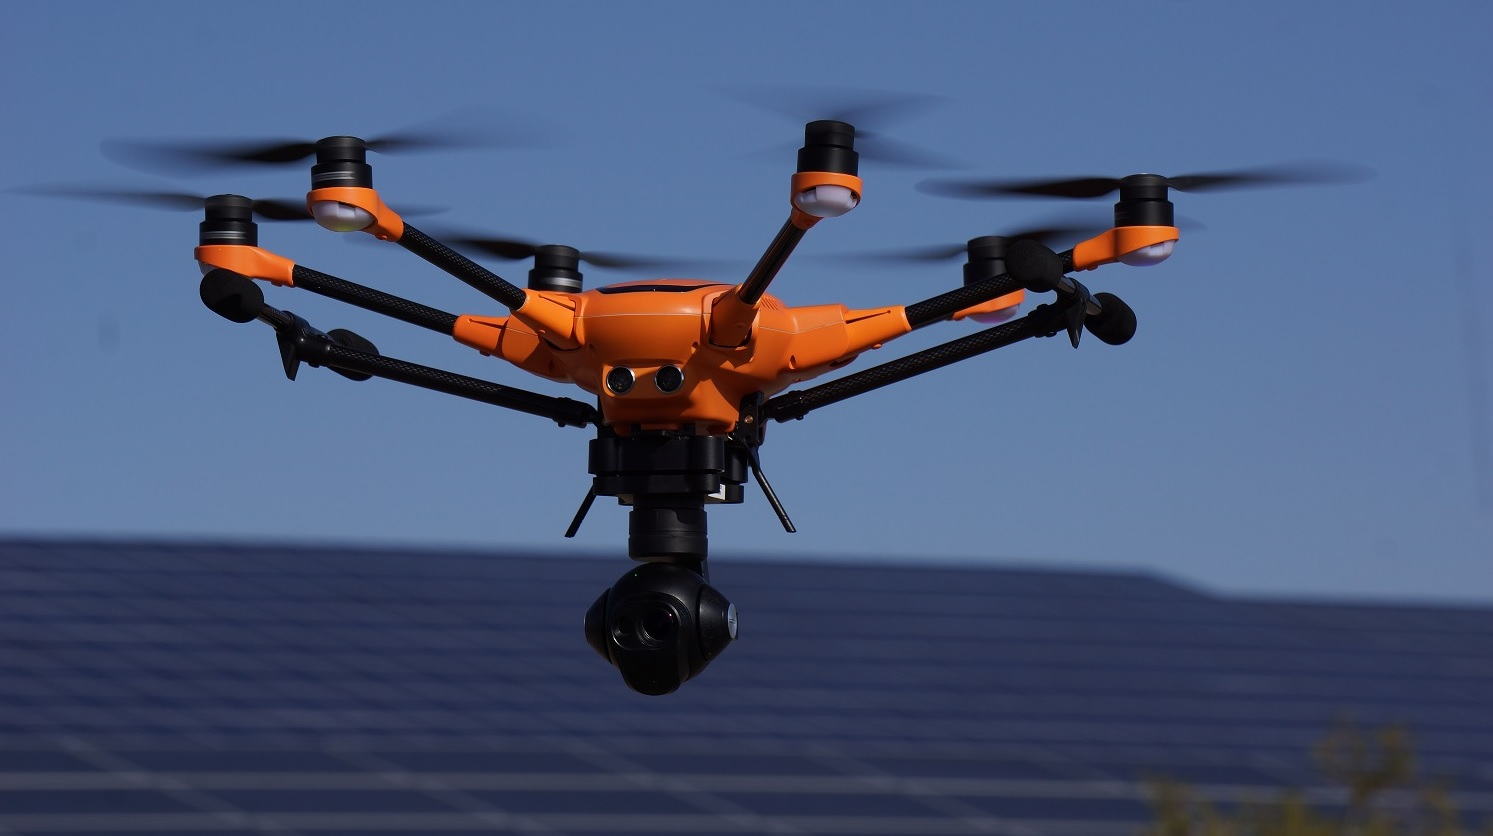
\includegraphics[width=0.6\textwidth]{multicopter.png}
            \caption{multicottero}
        \end{figure} 
        
        \column{0.48\textwidth}
        \textbf{Ala Fissa}
        \begin{itemize}
            \item[{\textcolor{green}{\checkmark}}] Alta efficienza, Lungo raggio.
            \item[{\textcolor{red}{$\times$}}] Necessità piste, No hovering.
        \end{itemize}
        \centering
        \begin{figure}
            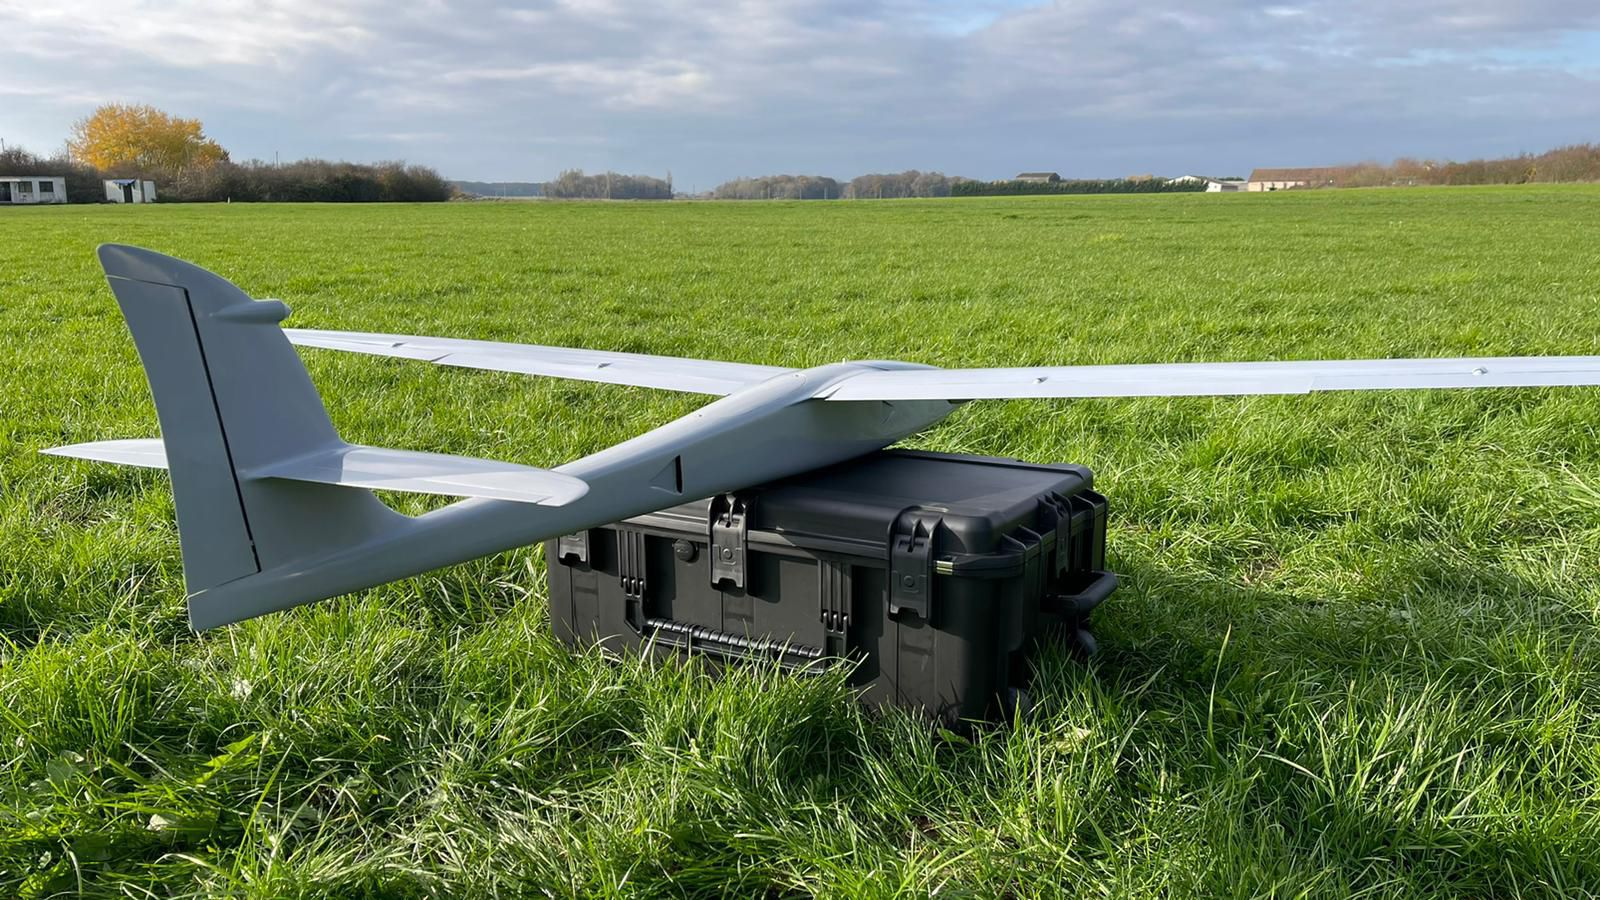
\includegraphics[width=0.6\textwidth]{fixed_wing.png}
            \caption{aereo}
        \end{figure}       
    \end{columns}

    % \vspace{0.2cm}
    \centering
    \textbf{Soluzione:} Configurazione Ibrida (VTOL)
\end{frame}

\begin{frame}{Il Concept VTOL Tilt-Rotor}
    Il tricottero \textit{Tilt-Rotor} combina i benefici delle due architetture:
    
    \begin{columns}
        \column{0.6\textwidth}
        \begin{itemize}
            \item \textbf{Decollo/Atterraggio:} Verticale (come un elicottero), indipendente da infrastrutture.
            \item \textbf{Crociera:} Volo aerodinamico (come un aereo) ruotando i propulsori.
        \end{itemize}
        
        \vspace{0.5cm}
        \begin{block}{La Sfida Ingegneristica}
            Questa versatilità introduce una \textbf{dinamica complessa} e fortemente accoppiata, 
            richiedendo strategie di controllo e allocazione avanzate.
        \end{block}

        \column{0.4\textwidth}
        \centering
        % Qui ci va l'immagine del TUO drone o un render CAD
        % Usa [draft] se non hai ancora l'immagine per vedere il riquadro vuoto
        \begin{figure}
            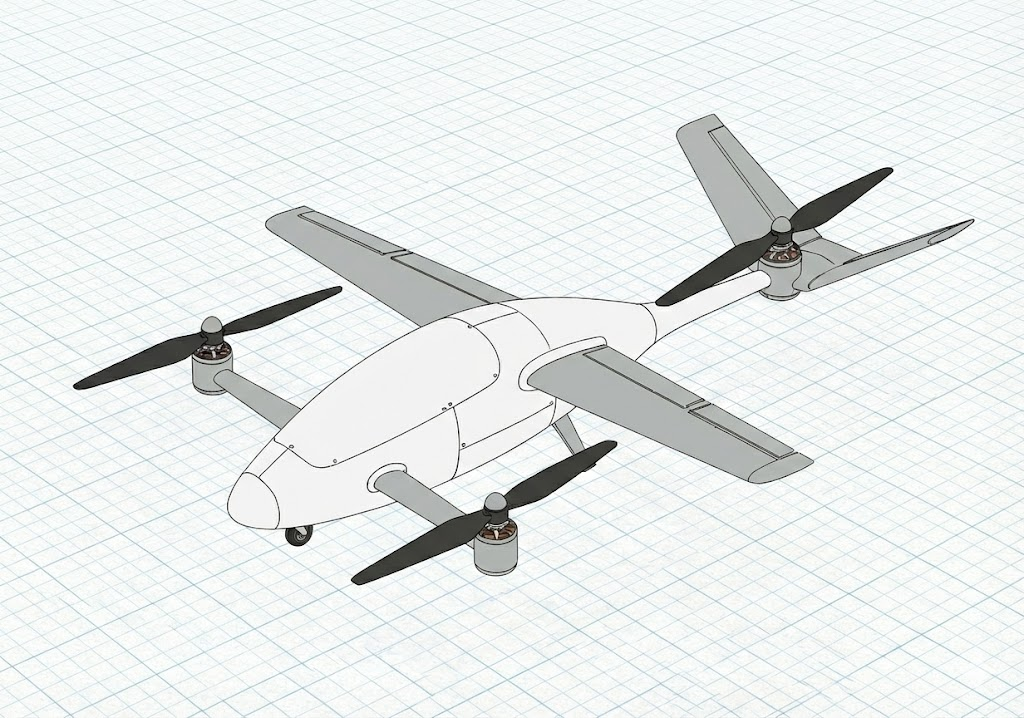
\includegraphics[width=0.8\textwidth]{VTOL.png}
            \caption{\footnotesize Rendering del velivolo.}
        \end{figure}
        
    \end{columns}
\end{frame}

\begin{frame}{La Soluzione: Tricottero Tilt-Rotor VTOL}
    Il velivolo proposto combina i vantaggi delle due architetture grazie alla capacità di \textbf{orientare i propulsori (Tilt)}.
        \begin{itemize}
            \item \textbf{Modalità Elicottero:} Decollo e atterraggio verticale.
            \item \textbf{Modalità Aereo:} I rotori ruotano per generare spinta orizzontale (transizione).
        \end{itemize}
        
        \vspace{0.4cm}
        \begin{block}{La Sfida Ingegneristica}
            Il sistema è \textbf{sottoattuato} in alcune fasi e presenta forti non-linearità e accoppiamenti dinamici.
        \end{block}
\end{frame}

% ============================================================
% 2. MODELLAZIONE
% ============================================================
\section{Modellazione Dinamica}

\begin{frame}{Sistemi di Riferimento}
    \small % Riduco leggermente il testo per far stare tutto
    Per descrivere la dinamica si adottano due sistemi destrorsi:
    
    \begin{itemize}
        \item \textbf{Sistema Inerziale ($\mathcal{F}_g$):} 
        Posizione $P_g = [x, y, z]^T$, Angoli $\Theta = [\phi, \theta, \psi]^T$.
        \item \textbf{Sistema Solidale ($\mathcal{F}_b$):}
        Origine nel CoM. $V_b = [u, v, w]^T$, $\Omega_b = [p, q, r]^T$.
    \end{itemize}   

    % --- INIZIO FIGURA FLOTTANTE ---
    \begin{figure}[htbp] 
        \centering
        % Usiamo le colonne PER L'IMPAGINAZIONE dentro la figura
        \begin{columns}[T]
            
            % Sotto-figura 1
            \begin{column}{0.48\textwidth}
                \centering
                \begin{subfigure}{\linewidth}
                    \centering
                    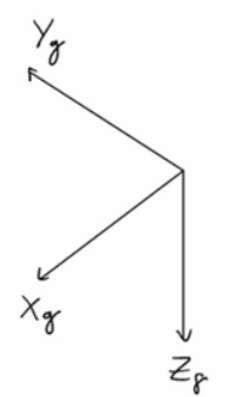
\includegraphics[height=3cm]{sist_rif_global.png} 
                    \caption{Sistema Globale}
                    \label{fig:global}
                \end{subfigure}
            \end{column}
            
            % Sotto-figura 2
            \begin{column}{0.48\textwidth}
                \centering
                \begin{subfigure}{\linewidth}
                    \centering
                    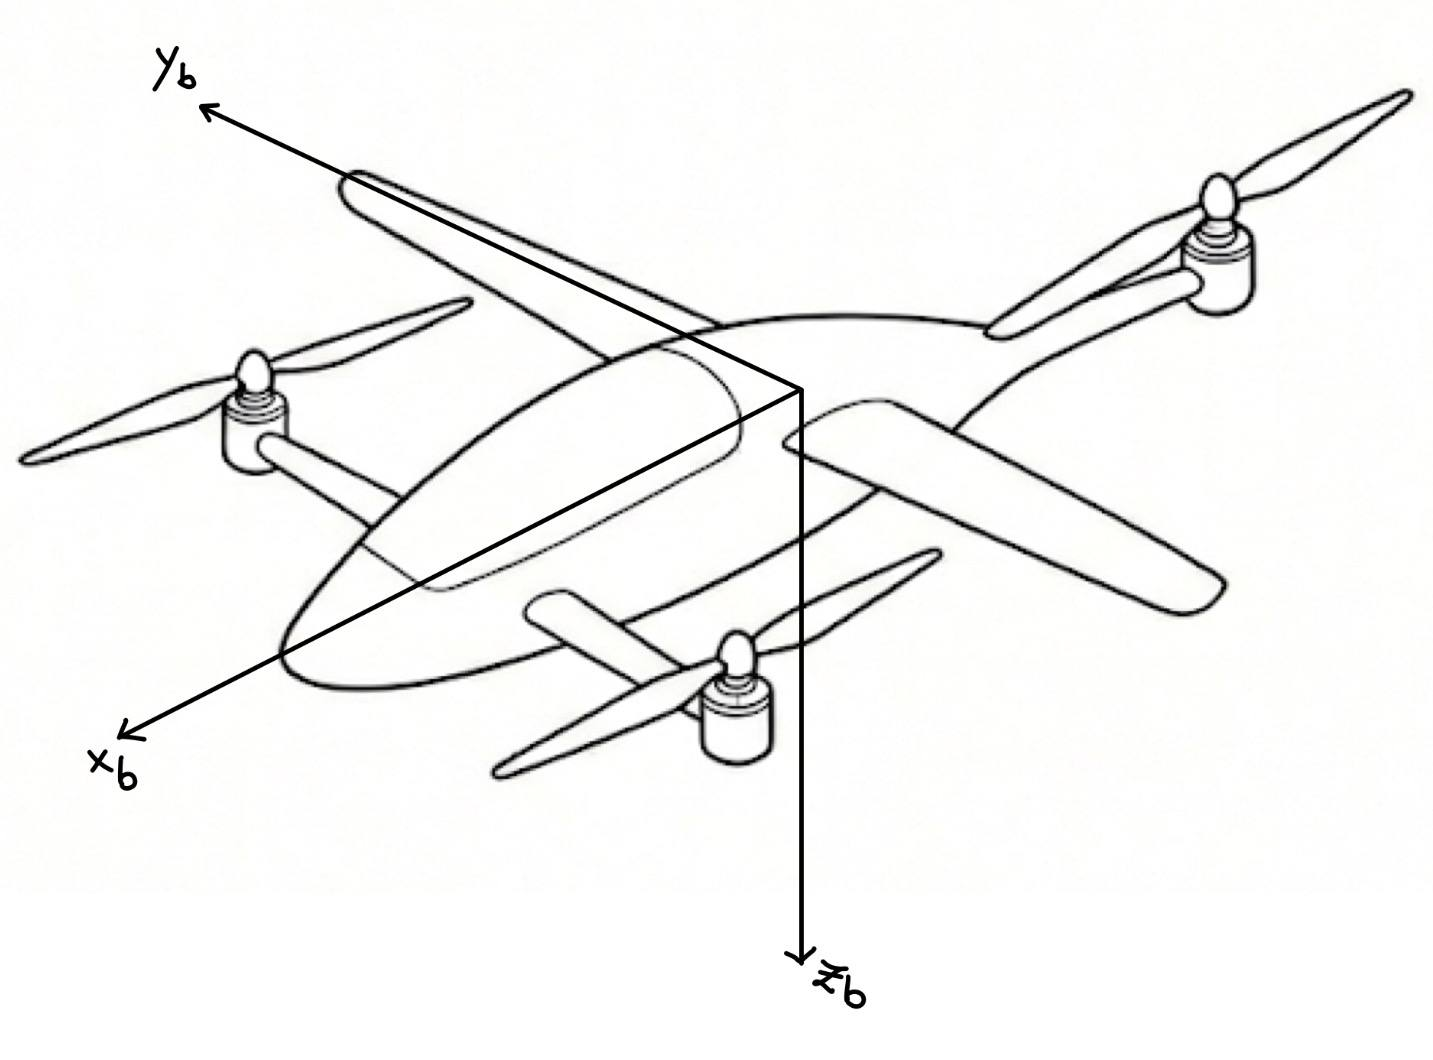
\includegraphics[height=3cm]{sist_rif_body.jpg}
                    \caption{Sistema Body}
                    \label{fig:body}
                \end{subfigure}
            \end{column}
            
        \end{columns}
        
        % Didascalia principale (che avrà il numero, es: Figure 1)
        \caption{Rappresentazione dei sistemi di riferimento inerziale e solidale.}
        \label{fig:sistemi_rif}
    \end{figure}
\end{frame}

\begin{frame}{Sistemi di Riferimento}
    Equazioni che legano velocità lineari e angolari nei due sistemi di riferimento:
    \begin{equation}
        \bm{\dot{P}}_{g} = R_{b \to g} \bm{V}_{b}
    \end{equation}
    \begin{equation}
        \bm{\dot{\Theta}}_{g} = J_{b \to g} \bm{\Omega}_{b}
    \end{equation}
    % Assicurati di avere \usepackage{bm} nel preambolo

    \begin{gather}
        \begin{bmatrix}
            \bm{\dot{P}}_g \\    % Il punto sopra rimane, il simbolo diventa bold
            \bm{\dot{\Theta}}_g
        \end{bmatrix}
        =
        \begin{bmatrix}
            R_{b \to g} & 0 \\    % Nota: ho aggiunto & per separare le colonne
            0 & J_{b \to g}
        \end{bmatrix}
        \begin{bmatrix}
            \bm{V}_b \\
            \bm{\Omega}_b
        \end{bmatrix}
    \end{gather}
\end{frame}

\begin{frame}{Configurazione Geometrica dei Rotori}
    Rispetto al modello standard, i rotori anteriori sono posizionati \textbf{avanzati} rispetto al Centro di Massa (CoM).
    
    \begin{columns}[c]
        \begin{column}{0.55\textwidth}
            \textbf{Vettori Posizione (Bracci):}
            \small
            \begin{itemize}
                \item \textbf{Rotore 1 (DX):} 
                $$ \bm{r}_1 = [d_x, d_y, 0]^T $$
                \item \textbf{Rotore 2 (SX):} 
                $$ \bm{r}_2 = [d_x, -d_y, 0]^T $$
                \item \textbf{Rotore 3 (Coda):} 
                $$ \bm{r}_3 = [-d_{tail}, 0, 0]^T $$
            \end{itemize}
            
            \vspace{0.2cm}
            \footnotesize
            \textcolor{red}{\textbf{Implicazione Dinamica:}} Poiché $d_x > 0$, la spinta dei rotori anteriori genera un momento di Pitch ($\tau_y$) anche a tilt nullo, accoppiando fortemente il moto verticale con quello longitudinale.
        \end{column}
        
        \begin{column}{0.45\textwidth}
            \centering
            % Inserisci qui la tua foto nuova o uno schema fatto con TikZ
            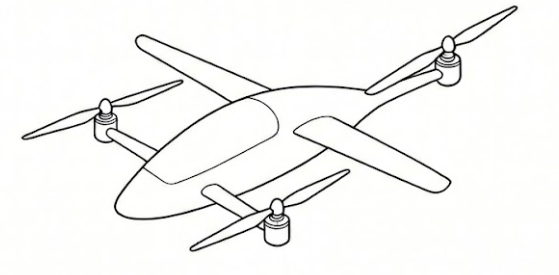
\includegraphics[width=\linewidth]{tricopter_2D.png}
            \captionof{figure}{\tiny Configurazione con rotori avanzati.}
        \end{column}
    \end{columns}
\end{frame}

\begin{frame}{Analisi delle Forze e Attuazione}
    Il tricottero dispone di 3 motori con gradi di libertà di tilt:
    
    \vspace{0.2cm}
    \begin{columns}
        \column{0.5\textwidth}
        \centering
        \textbf{Rotori Anteriori}
        % SOSTITUISCI CON 'rotori_1_2.png'
        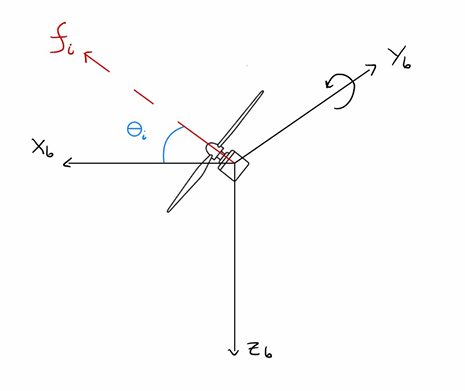
\includegraphics[width=0.7\textwidth]{rotori_1_2.png}
        \vspace{0.2cm}\\
        \footnotesize{Tilt attorno all'asse $Y_b$.}
        
        \column{0.5\textwidth}
        \centering
        \textbf{Rotore di Coda}
        % SOSTITUISCI CON 'rotore_3.png'
        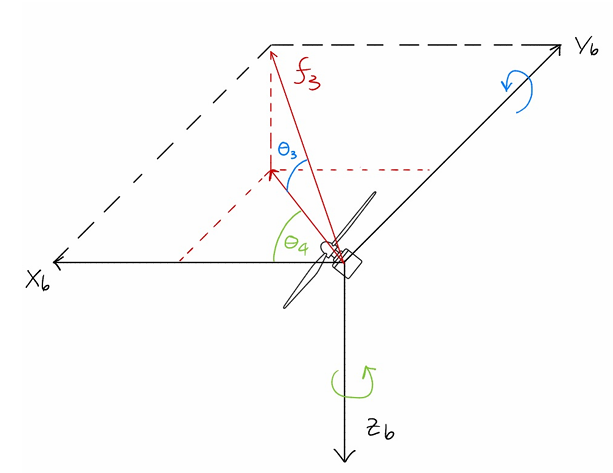
\includegraphics[width=0.7\textwidth]{rotore_3.png}
        \vspace{0.25cm}\\
        \footnotesize{Tilt su $Y_b$ e $Z_b$.}
    \end{columns}
    
    \vspace{0.3cm}
    % La dimensione del font deve avvolgere l'equazione, non starci dentro
    {\footnotesize 
    \begin{equation}
        F_{th} = \sum_{i=1}^{3} R_{tilt,i} \cdot T_i \quad \text{(Forza propulsiva nel body frame)}
    \end{equation}
    }
\end{frame}

% --- Frame 2: Equazioni (Tuo Codice) ---
\begin{frame}{Equazioni della Dinamica}
    Modello Newton-Eulero per corpo rigido a 6 gradi di libertà:
    
    \begin{block}{Equazioni Vettoriali}
    \begin{equation}
        \begin{cases}
            m \dot{V}_b + \Omega_b \times (m V_b) = F_{\mathrm{tot}} \\
            I_b \dot{\Omega}_b + \Omega_b \times (I_b \Omega_b) = M_{\mathrm{tot}}
        \end{cases}
    \end{equation}
    \end{block}
    
    Dove:
    \begin{itemize}
        \item $F_{\mathrm{tot}} = F_{\mathrm{th}} + F_g + F_{\mathrm{aero}}$
        \item $M_{\mathrm{tot}} = M_{\mathrm{th}} + M_{\mathrm{aero}} + M_{\mathrm{gyro}} + M_{\mathrm{pinna}}$
    \end{itemize}
\end{frame}

\begin{frame}{Dinamica Traslazionale (Forze Aerodinamiche)}
    La dinamica include le forze aerodinamiche che agiscono sulle superfici alari e sulla fusoliera.

    \begin{columns}[c]
        % --- COLONNA EQUAZIONI ---
        \begin{column}{0.55\textwidth}
            La forza totale è data da:
            $$ m \bm{\dot{V}}_b = \bm{F}_{th} + \bm{F}_{g} + \bm{F}_{aero} - \bm{\Omega}_b \times (m \bm{V}_b) $$
            
            Modello aerodinamico semplificato:
            \footnotesize
            \begin{equation*}
                \bm{F}_{aero} \approx 
                \begin{bmatrix}
                     -\frac{1}{2}\rho S (C_D +D_D) v_x |v_x| \\
                     0 \\
                     -\frac{1}{2}\rho S (C_L + C_L) v_x^2
                \end{bmatrix}
            \end{equation*}
            \tiny
            Dove $C_x$ include la resistenza parassita e $C_z$ la resistenza verticale in hovering.
        \end{column}

        % --- COLONNA IMMAGINE ---
        \begin{column}{0.45\textwidth}
            \centering
            % Sostituisci con il nome del file caricato (quello con le frecce rosse e blu)
            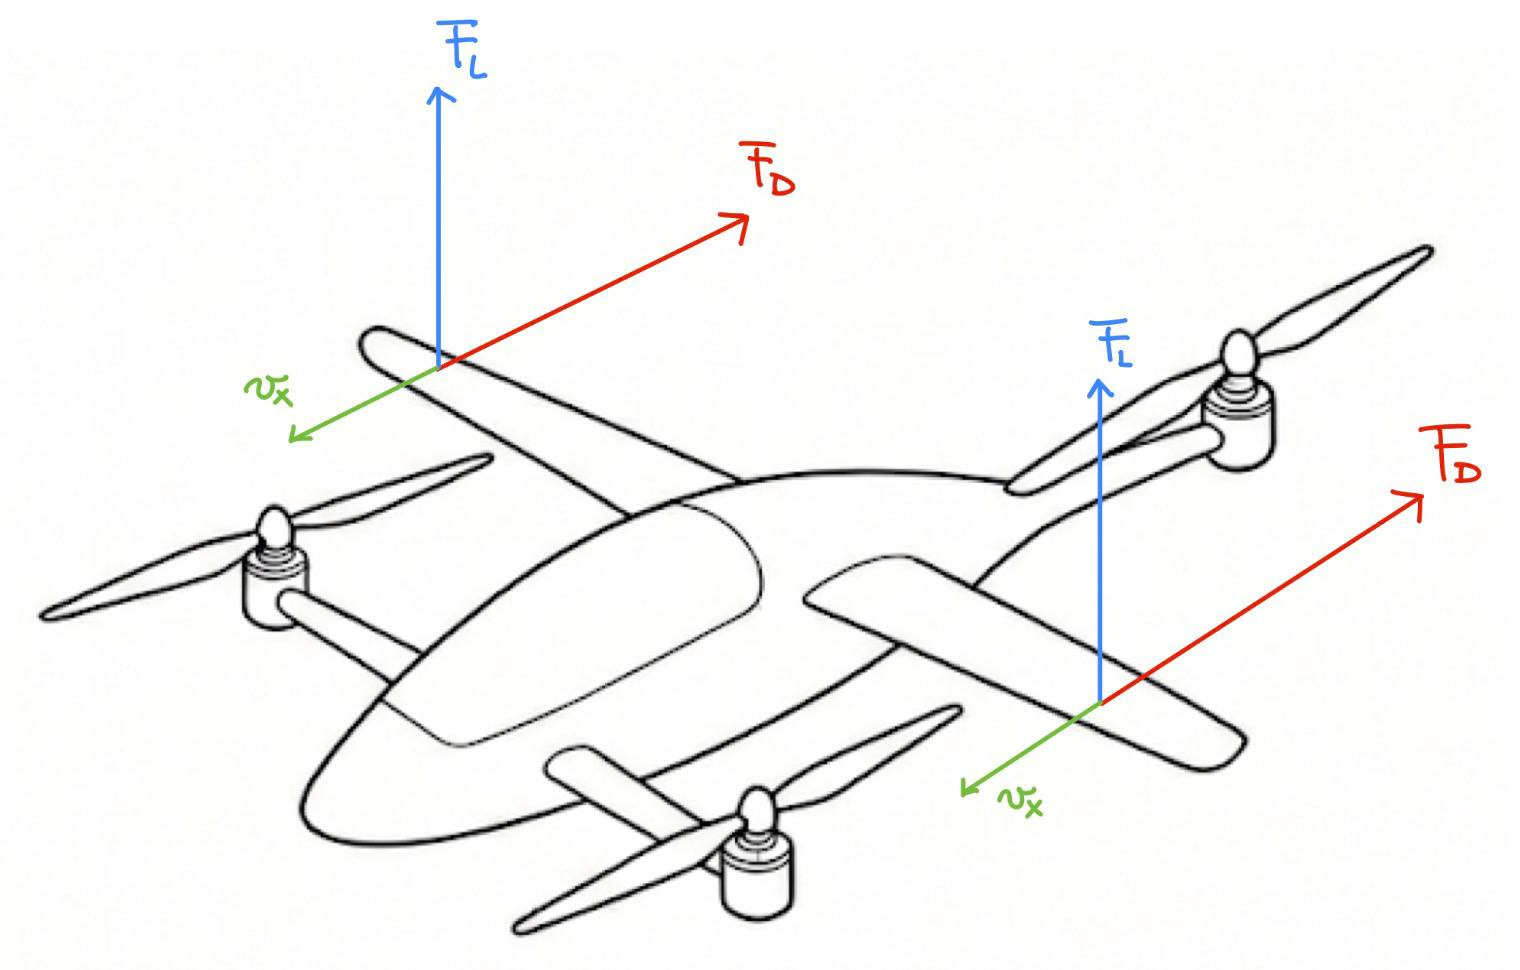
\includegraphics[width=\linewidth]{forze_x.jpg}
            \captionof{figure}{\tiny Scomposizione forze: Lift ($F_L$) e Drag ($F_D$).}
        \end{column}
    \end{columns}
\end{frame}

% \begin{frame}{Dinamica Verticale (Asse Z)}
%     L'equazione del moto lungo l'asse $Z_b$ è critica per l'hovering e il mantenimento della quota. 
    
%     $$ m \dot{w} = F_{th,z} + F_{g,z} + F_{aero,z} + \Delta_{coriolis} $$

%     \begin{columns}[c]
%         % --- COLONNA MATEMATICA ---
%         \begin{column}{0.55\textwidth}
%             \textbf{Componenti delle Forze:}
%             \footnotesize
%             \begin{itemize}
%                 \item \textbf{Thrust Verticale ($F_{th,z}$):} 
%                 Dipende dal tilt dei rotori. In hovering ($\theta \approx 90^\circ$):
%                 $$ F_{th,z} \approx -(f_1 + f_2 + f_3) $$
%                 \item \textbf{Gravità ($F_{g,z}$):}
%                 Proiezione del peso sugli assi body:
%                 $$ F_{g,z} = mg \cos\theta \cos\phi $$
%                 \item \textbf{Resistenza Verticale ($F_{D_z}$):}
%                 La fusoliera oppone resistenza al moto verticale (effetto "piastra piana"):
%                 \begin{equation}
%                     F_{D_z} = -\frac{1}{2} \rho S_{top} C_{D_z} w |w|
%                 \end{equation}
%             \end{itemize}
%         \end{column}

%         % --- COLONNA VISUALE ---
%         \begin{column}{0.45\textwidth}
%             \centering
%             % Immagine specifica per l'asse Z che hai caricato
%             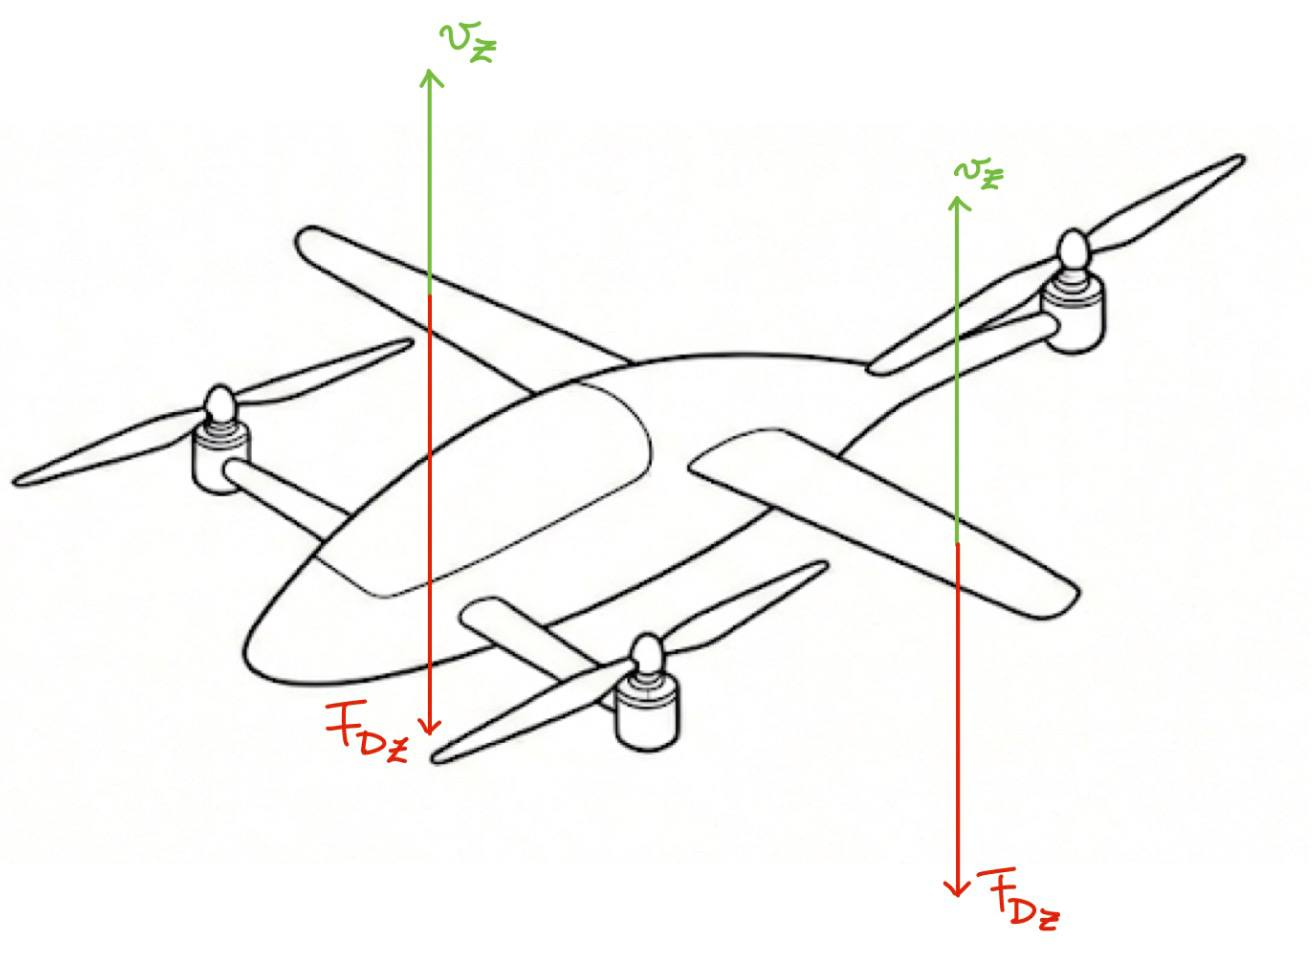
\includegraphics[width=\linewidth]{forze_z.jpg}
%             \captionof{figure}{\tiny Relazione tra velocità verticale ($v_z$) e resistenza ($F_{D_z}$).}
%         \end{column}
%     \end{columns}
    
%     \vspace{0.2cm}
%     \tiny
%     \textit{Nota: Il termine $F_{D_z}$ agisce come smorzamento naturale, stabilizzando la discesa ma richiedendo extra potenza in salita.}
% \end{frame}


\begin{frame}{Dinamica Rotazionale (Momenti)}
    L'evoluzione dell'assetto è governata dalla legge di Eulero:
    $$ I_b \bm{\dot{\Omega}}_b + \bm{\Omega}_b \times (I_b \bm{\Omega}_b) = \bm{M}_{tot} $$
    
    Il momento totale agente sul tricottero è la somma di quattro contributi:
    \begin{equation}
        \bm{M}_{tot} = \bm{M}_{th} + \bm{M}_{aero} + \bm{M}_{gyro} + \bm{M}_{pinna}
    \end{equation}

    \vspace{0.1cm}
    \begin{columns}[T]
        % --- COLONNA SINISTRA: Il termine di Controllo (Thrust) ---
        \begin{column}{0.55\textwidth}
            \textbf{1. Momenti Propulsivi ($\bm{M}_{th}$):}
            \tiny
            \begin{equation*}
                \bm{M}_{th} \approx 
                \begin{bmatrix}
                    d_y (F_{z,1} - F_{z,2}) + M_{roll,tilt} \\
                    \underbrace{-d_x (F_{z,1} + F_{z,2}) + d_{tail} F_{z,3}}_{\text{Bilanciamento Pitch}} + M_{pitch,tilt} \\
                    d_x (F_{y,1} + F_{y,2}) + d_y (F_{x,2} - F_{x,1}) + M_{yaw}
                \end{bmatrix}
            \end{equation*}
        \end{column}
        
        % --- COLONNA DESTRA: I Disturbi/Effetti Secondari ---
        \begin{column}{0.45\textwidth}
            \textbf{Altri Contributi:}
            \footnotesize
            \begin{itemize}
                \item $\bm{M}_{aero}$: Resistenza aerodinamica rotazionale (drag angolare).
                \item $\bm{M}_{gyro}$: Effetti giroscopici dovuti alla rotazione rapida delle eliche e al loro tilt.
                \item $\bm{M}_{pinna}$: Momento stabilizzante generato dalla deriva di coda (Yaw damping naturale).
            \end{itemize}
        \end{column}
    \end{columns}
    
    \vspace{0.2cm}
    \tiny
    \textit{Nota: Nel controllo, $\bm{M}_{th}$ è l'input, mentre gli altri termini sono trattati come disturbi da compensare o smorzamenti naturali.}
\end{frame}

% --- SLIDE DETTAGLIO 1: AERODINAMICA ---
\begin{frame}{Dettaglio: Momento Aerodinamico ($\bm{M}_{aero}$)}
    Le superfici alari non generano solo forze, ma anche momenti dovuti al fatto che il Centro di Pressione (CP) non coincide con il CoM.
    
    $$ \bm{M}_{aero} = \sum_{i \in \{dx, sx\}} \bm{r}_{cp,i} \times \bm{F}_{aero,i} $$
    
    Espandendo il prodotto vettoriale per l'ala destra e sinistra:
    \footnotesize
    \begin{equation*}
        \bm{M}_{aero} \approx
        \begin{bmatrix}
            l_{y} (F_{z,sx} - F_{z,dx}) \\
            l_{x} (F_{z,dx} + F_{z,sx}) + l_{z} (F_{x,dx} + F_{x,sx}) \\
            l_{y} (F_{x,dx} - F_{x,sx})
        \end{bmatrix}
    \end{equation*}
    
    \normalsize
    \begin{block}{Effetto Fisico}
    Durante il volo avanzato ($v_x > 0$), questo termine introduce uno \textbf{smorzamento aerodinamico} e un momento di beccheggio che tende a "raddrizzare" il drone.
    \end{block}
\end{frame}

\begin{frame}{Dettaglio: Momento Giroscopico ($\bm{M}_{gyro}$)}
    Il momento giroscopico nasce dall'interazione tra la rotazione veloce dei propulsori ($\omega_i$) e la velocità di tilting ($\dot{\theta}_i$). 
    
    Dall'equazione (3.42), la matrice dei momenti giroscopici totali è:

    \footnotesize
    \begin{equation}
        \bm{M}_{gyro} = \sum_{i=1}^{3} \bm{I}_{rot,i} (\bm{\Omega}_{i} \times \bm{\Omega}_{tilt,i}) = 
        \begin{bmatrix}
             I_{zz} \dot{\theta}_1 \sin\theta_1 \omega_1 + I_{zz} \dot{\theta}_2 \sin\theta_2 \omega_2 + (\dots)_3 \\
             0 \\
             I_{zz} \dot{\theta}_1 \cos\theta_1 \omega_1 + I_{zz} \dot{\theta}_2 \cos\theta_2 \omega_2 + (\dots)_3
        \end{bmatrix}
    \end{equation}
    
    \vspace{0.2cm}
    \textbf{Dove per il rotore di coda ($i=3$) con 2 DoF:}
    \scriptsize
    \begin{equation*}
       (\dots)_3 = \text{Termini accoppiati dipendenti da } \dot{\theta}_3, \dot{\theta}_4 \text{ e } \sin\theta_3, \cos\theta_4
    \end{equation*}

    \vspace{0.3cm}
    \normalsize
    \begin{alertblock}{Significato Fisico}
    Questi termini non sono nulli solo durante la \textbf{transizione} ($\dot{\theta} \neq 0$). 
    Ad esempio, il termine $I_{zz} \dot{\theta}_1 \sin\theta_1 \omega_1$ rappresenta un momento di rollio indotto dal tilt del rotore destro.
    \end{alertblock}
\end{frame}

% --- SLIDE DETTAGLIO 3: PINNA ---
\begin{frame}{Dettaglio: Stabilizzazione Passiva (Pinna)}
    La deriva di coda (Vertical Fin) genera un momento aerodinamico che si oppone alle rotazioni, garantendo stabilità passiva in volo avanzato.
    
    $$ \bm{M}_{pinna} = \bm{r}_{pinna} \times \bm{F}_{lat} $$
    
    Modello semplificato lineare:
    \begin{equation}
        \bm{M}_{pinna} = 
        \begin{bmatrix}
            - \alpha_{roll} \cdot p \cdot v_{fwd}^2 \\
            0 \\
            - \alpha_{yaw} \cdot r \cdot v_{fwd}^2
        \end{bmatrix}
    \end{equation}
    
    \vspace{0.2cm}
    \small
    \textbf{Funzione:} Agisce come uno "smorzatore naturale" (Damper) per il Rollio ($p$) e l'Imbardata ($r$). All'aumentare della velocità $v_{fwd}$, il drone diventa naturalmente più stabile e meno sensibile ai disturbi laterali.
\end{frame}

% ============================================================
% 3. ARCHITETTURA DI CONTROLLO
% ============================================================
\section{Architettura di Controllo}

\begin{frame}{Configurazione fase di decollo}
    La prima fase di volo è quella di decollo verticale, durante la quale i motori sono posizionati verticalmente per generare una propulsione in grado di far sollevare il drone.
    
    \vspace{0.3cm}
    Si assume che in tale posizione gli angoli di tilt siano i seguenti:
    \begin{itemize}
        \item $\theta_1 = \theta_2 = \pi/2$ (Rotori anteriori verticali).
        \item $\theta_4 = -\pi/2$ (Braccio di coda orientato lateralmente).
        \item $\theta_3 = \theta_{3,eq}$: tale angolo permette di contrastare il momento torcente attorno all'asse $z$ causato dalla coppia di reazione del motore posteriore, non essendo presente un secondo rotore controrotante per il bilanciamento.
    \end{itemize}
\end{frame}

% --- SLIDE 1: Panoramica Strategia ---
\begin{frame}{Architettura Gerarchica a Cascata}
    Sulla base dell'analisi dinamica, è stata implementata un'architettura di controllo a cascata che disaccoppia la dinamica lenta (posizione) da quella veloce (assetto).

    \begin{block}{Suddivisione Logica}
    \begin{enumerate}
        \item \textbf{Outer Loop (Posizione $x, y, z$):}
        Utilizza la tecnica \textbf{Sliding Mode Control (SMC)}.
        \begin{itemize}
            \item Calcola le forze richieste ($F_{req}$) per annullare l'errore di posizione.
            \item Effettua un \textit{mapping cinematico} traducendo le forze planari in angoli di assetto desiderati ($\phi_{des}, \theta_{des}$).
        \end{itemize}
        
        \item \textbf{Inner Loop (Assetto $\phi, \theta, \psi$):}
        Utilizza controllori \textbf{PID} per inseguire gli angoli desiderati calcolati dal loop esterno e stabilizzare le velocità angolari.
    \end{enumerate}
    \end{block}
    
    \vspace{0.2cm}
    \textbf{Peculiarità:} Il controllo di quota e quello planare sono \textbf{accoppiati}. La spinta totale $T$ (loop $z$) funge da termine di normalizzazione per determinare l'inclinazione del vettore spinta.
\end{frame}

% --- SLIDE 2: Schema a Blocchi (Codice TikZ fornito) ---
\begin{frame}
    \begin{figure}[htbp]
        \centering
        % Resizebox adatta il diagramma alla larghezza del testo
        \resizebox{0.8\textwidth}{!}{
        \begin{tikzpicture}[auto, node distance=1.5cm, >=latex']
            % --- STILI ---
            \tikzstyle{block} = [draw, rectangle, minimum height=3em, minimum width=3.5em, align=center, fill=white]
            \tikzstyle{sum} = [draw, circle, inner sep=0mm, minimum size=6mm, node distance=1.5cm]
            \tikzstyle{input} = [coordinate]
            \tikzstyle{output} = [coordinate]
            \tikzstyle{container} = [draw, rectangle, rounded corners, dashed, inner sep=0.3cm, black!60]
        
            % --- 1. RIGA: QUOTA (Z) ---
            \node [input] (ref_z) {};
            \node [sum, right of=ref_z, node distance=1cm] (sum_z) {$\Sigma$};
            \node [block, right of=sum_z, node distance=2.5cm] (smc_z) {SMC\\Quota $z$};
            \node [left of=ref_z, node distance=0.8cm] {$\mathbf{z_{ref}}$}; 
        
            % --- 2. RIGA: POSIZIONE Y -> ROLL (PHI) ---
            \node [input, below of=ref_z, node distance=2.5cm] (ref_y) {};
            \node [sum, right of=ref_y, node distance=1cm] (sum_y) {$\Sigma$};
            \node [block, right of=sum_y, node distance=2.5cm] (smc_phi) {SMC\\$y \to \phi$};
            \node [sum, right of=smc_phi, node distance=2.5cm] (sum_roll) {$\Sigma$};
            \node [block, right of=sum_roll, node distance=2cm] (pid_roll) {PID\\ROLL};
            \node [left of=ref_y, node distance=0.8cm] {$\mathbf{y_{ref}}$};
        
            % --- 3. RIGA: POSIZIONE X -> PITCH (THETA) ---
            \node [input, below of=ref_y, node distance=2.5cm] (ref_x) {};
            \node [sum, right of=ref_x, node distance=1cm] (sum_x) {$\Sigma$};
            \node [block, right of=sum_x, node distance=2.5cm] (smc_theta) {SMC\\$x \to \theta$};
            \node [sum, right of=smc_theta, node distance=2.5cm] (sum_pitch) {$\Sigma$};
            \node [block, right of=sum_pitch, node distance=2cm] (pid_pitch) {PID\\PITCH};
            \node [left of=ref_x, node distance=0.8cm] {$\mathbf{x_{ref}}$};
        
            % --- 4. RIGA: YAW (PSI) ---
            \node [input, below of=ref_x, node distance=2.5cm] (ref_psi) {};
            \node [sum, right of=ref_psi, node distance=1cm] (sum_yaw) {$\Sigma$};
            \node [block] at (pid_pitch |- sum_yaw) (pid_yaw) {PID\\YAW}; 
            \node [left of=ref_psi, node distance=0.8cm] {$\mathbf{\psi_{ref}}$};
        
            % --- MIXER E DRONE ---
            \node [block, minimum height=8cm, text width=1.5cm, right of=pid_pitch, xshift=2.5cm, yshift=1.25cm] (mixer) {MIXER};
            \node [block, right of=mixer, node distance=3.5cm, minimum height=5cm] (drone) {DRONE};
        
            % --- COLLEGAMENTI FORWARD ---
            
            % Z Loop
            \draw [->] (ref_z) -- (sum_z);
            \draw [->] (sum_z) -- node[above, font=\footnotesize] {$e_z$} (smc_z);
            
            % --- CONNESSIONE THRUST (Correzione Rigorosa) ---
            
            % 1. Definiamo una "x" sicura per il bus verticale (a metà precisa tra le colonne)
            \coordinate (bus_x) at ($(sum_y.east)!0.5!(smc_phi.west)$);
            
            % 2. Disegniamo la linea principale che scende
            % Parte da SMC_Z, va giù un po', gira a sinistra fino al bus_x, poi scende fino all'ultimo blocco
            \draw [->] (smc_z.south) -- ++(0,-0.2) -| (bus_x) -- (bus_x |- smc_theta.south);
            
            % Etichetta F_req,z posizionata meglio (sopra il primo tratto orizzontale)
            \node[above, font=\footnotesize] at ($(smc_z.south) + (-1, -0.2)$) {$F_{req,z}$};

            % 3. Collegamento a SMC Phi (Ingresso dall'alto pulito)
            % Partiamo dal bus all'altezza del blocco -> SALIAMO -> ENTRIAMO da sopra
            \draw [->] (bus_x |- smc_phi.north) -- ++(0, 0.3) -| (smc_phi.north);

            % 4. Collegamento a SMC Theta (Ingresso dall'alto pulito)
            \draw [->] (bus_x |- smc_theta.north) -- ++(0, 0.3) -| (smc_theta.north);
            % Y -> Phi Loop
            \draw [->] (ref_y) -- (sum_y);
            \draw [->] (sum_y) -- node[above, font=\footnotesize] {$e_y$} (smc_phi);
            \draw [->] (smc_phi) -- node[above, font=\footnotesize] {$\phi_{des}$} (sum_roll);
            \draw [->] (sum_roll) -- node[above, font=\footnotesize] {$e_\phi$} (pid_roll);
            \draw [->] (pid_roll) -- node[above, near end, font=\footnotesize] {$M_x$} (mixer.west |- pid_roll);
        
            % X -> Theta Loop
            \draw [->] (ref_x) -- (sum_x);
            \draw [->] (sum_x) -- node[above, font=\footnotesize] {$e_x$} (smc_theta);
            \draw [->] (smc_theta) -- node[above, font=\footnotesize] {$\theta_{des}$} (sum_pitch);
            \draw [->] (sum_pitch) -- node[above, font=\footnotesize] {$e_\theta$} (pid_pitch);
            \draw [->] (pid_pitch) -- node[above, near end, font=\footnotesize] {$M_y$} (mixer.west |- pid_pitch);
        
            % Yaw Loop
            \draw [->] (ref_psi) -- (sum_yaw);
            \draw [->] (sum_yaw) -- node[above, font=\footnotesize] {$e_\psi$} (pid_yaw);
            \draw [->] (pid_yaw) -- node[above, near end, font=\footnotesize] {$M_z$} (mixer.west |- pid_yaw);
        
            % Mixer -> Drone
            \draw [->] (mixer) -- (drone);
        
            % --- FEEDBACK LOOP ---
            \draw [->] (drone.east) -- ++(1,0) coordinate (fb_start) 
                -- ++(0,-5.5) coordinate (fb_corner) 
                -- (fb_corner -| sum_z) coordinate (fb_end) -- ++(-1,0); 
        
            % Feedback salite (PULITE: Senza etichette e segni meno)
            \draw [->] (fb_end -| sum_z) -- (sum_z.south);
            \draw [->] (fb_end -| sum_y) -- (sum_y.south);
            \draw [->] (fb_end -| sum_x) -- (sum_x.south);
            \draw [->] (fb_end -| sum_yaw) -- (sum_yaw.south);
            \draw [->] (fb_end -| sum_roll) -- (sum_roll.south);
            \draw [->] (fb_end -| sum_pitch) -- (sum_pitch.south);
                
            % Etichetta feedback centrata
            \node [below] at ($(fb_corner)!0.5!(fb_end)$) {Stato $\mathbf{x}$ (Feedback)};
        
            % --- RIQUADRI LOGICI ---
            \node [container, fit=(smc_z) (smc_phi) (smc_theta), label=above:\textbf{Outer Loop: Posizione}] {};
            \node [container, fit=(pid_roll) (pid_pitch) (pid_yaw), label=above:\textbf{Inner Loop: Assetto}] {};
        
        \end{tikzpicture}
        } % Chiusura resizebox
        \caption{Schema a blocchi del controllo verticale.}
        \label{fig:control_scheme_vertical}
    \end{figure}
\end{frame}

% --- SLIDE 3: Controllo Verticale (SMC) ---
\begin{frame}{Controllo di Quota (Outer Loop)}
    
    \begin{columns}[T]
        % --- COLONNA SINISTRA: Matematica ---
        \begin{column}{0.6\textwidth}
            \textbf{Obiettivo:} Robustezza ai disturbi.
            
            \vspace{0.2cm}
            \textbf{1. Definizioni:}
            \begin{itemize}
                \item Errore: $e_z = z_{des} - z$
                \item Superficie: $\sigma_z = \dot{e}_z + \lambda_z e_z$
            \end{itemize}
            
            \vspace{0.3cm}
            \textbf{2. Legge di Controllo ($F_{req,z}$):}
            \begin{equation*}
                 \underbrace{mg + F_{aero,z} - m \lambda_z \dot{e}_z}_{\text{Linearizzazione}} - \underbrace{m K_z \tanh\left(\frac{\sigma_z}{\Phi}\right)}_{\text{Termine Robusto}}
            \end{equation*}
            
            \vspace{0.2cm}
            \small
            L'uso di $\tanh(\cdot)$ al posto di $\text{sgn}(\cdot)$ definisce uno strato limite $\Phi$ per eliminare il \textit{chattering}.
        \end{column}
        
        % --- COLONNA DESTRA: Concetto Grafico ---
        \begin{column}{0.4\textwidth}
            \centering
            \vspace{0.5cm}
            \begin{tikzpicture}[scale=0.8, >=latex]
                % Assi
                \draw[->] (-2,0) -- (2,0) node[right] {$\sigma$};
                \draw[->] (0,-1.5) -- (0,1.5) node[above] {$u_{rob}$};
                
                % Funzione SIGN (Chattering) - Tratteggiata rossa
                \draw[red, dashed, thick] (-1.8,-1) -- (0,-1) -- (0,1) -- (1.8,1);
                \node[red, font=\scriptsize] at (1.5, 1.2) {sgn};
                
                % Funzione TANH (Smooth) - Blu solida
                \draw[blue, thick, domain=-1.8:1.8, samples=50] plot (\x, {tanh(2*\x)});
                \node[blue, font=\scriptsize] at (1.5, 0.6) {tanh};
                
                % Indicazione Boundary Layer
                \draw[<->, gray] (-0.5, -0.2) -- (0.5, -0.2);
                \node[gray, below, font=\tiny] at (0, -0.2) {$\Phi$};
            \end{tikzpicture}
            
            \vspace{0.2cm}
            \captionof{figure}{\footnotesize Smoothing dell'azione di controllo.}
        \end{column}
    \end{columns}
\end{frame}

\begin{frame}{Analisi di Stabilità (Metodo di Lyapunov)}
    
    Per garantire la stabilità asintotica globale della superficie di scorrimento ($\sigma \to 0$), si utilizza il criterio di Lyapunov.

    \vspace{0.3cm}
    
    \begin{columns}[T]
        % --- COLONNA SINISTRA: I Passaggi Logici ---
        \begin{column}{0.6\textwidth}
            \textbf{1. Funzione Candidata (Energia):}
            \begin{equation*}
                V(\sigma) = \frac{1}{2}\sigma^2 > 0
            \end{equation*}
            
            \textbf{2. Derivata Temporale:}
            Sostituendo la dinamica a ciclo chiuso con disturbo $\Delta$:
            \begin{align*}
                \dot{V} &= \sigma \dot{\sigma} \\
                        &= -k \sigma \text{sgn}(\sigma) + \sigma \Delta \\
                        &\le -k |\sigma| + |\sigma| \delta_{\max}
            \end{align*}
        \end{column}
        
        % --- COLONNA DESTRA: La Condizione ---
        \begin{column}{0.4\textwidth}
            \centering
            \vspace{1cm}
            \begin{alertblock}{Condizione di Stabilità}
                Affinché l'energia decresca ($\dot{V} < 0$), il guadagno deve "battere" il disturbo:
                \vspace{0.2cm}
                \centering
                \large
                \boldmath
                $k > \delta_{\max}$
                \unboldmath
            \end{alertblock}
            
            \vspace{0.3cm}
            \small \itshape
            Il sistema è robusto se il guadagno di switching supera il limite superiore dell'incertezza.
        \end{column}
    \end{columns}

    % Grafico concettuale opzionale in basso
    \vspace{0.5cm}
    \centering
    \begin{tikzpicture}[scale=0.6]
        \draw[->] (0,0) -- (6,0) node[right] {$t$};
        \draw[->] (0,0) -- (0,2.5) node[above] {$V(\sigma)$};
        \draw[thick, blue] plot [domain=0:5.5, samples=100] (\x, {2*exp(-\x)});
        \node[blue] at (2, 1.5) {$\dot{V} < 0$};
        \draw[dashed] (0,0) node[left] {0} -- (6,0);
    \end{tikzpicture}

\end{frame}

\begin{frame}{Gestione dei Disturbi e Tuning del Guadagno}
    
    Il vantaggio principale dello SMC è che non richiede la conoscenza puntuale del disturbo $d(t)$, ma solo del suo inviluppo massimo (Upper Bound).
    
    \begin{columns}[c]
        \begin{column}{0.5\textwidth}
            \textbf{Condizione di Robustezza:}
            $$ k > |\Delta(t)|_{\max} $$
            
            \vspace{0.2cm}
            \small
            \begin{itemize}
                \item \textcolor{green!60!black}{\textbf{Guadagno Ottimale:}} $k$ leggermente superiore al disturbo massimo atteso. Stabilità garantita e chattering ridotto.
                \item \textcolor{red}{\textbf{Guadagno Eccessivo:}} Stabilità garantita, ma forte chattering e stress sugli attuatori.
                \item \textcolor{orange}{\textbf{Guadagno Insufficiente:}} Il disturbo "rompe" il vincolo di sliding. Perdita di stabilità.
            \end{itemize}
        \end{column}
        
        \begin{column}{0.5\textwidth}
            \centering
            \begin{tikzpicture}[scale=0.8]
                % Assi
                \draw[->] (0,0) -- (5,0) node[right] {$t$};
                \draw[->] (0,-2.5) -- (0,2.5) node[above] {Ampiezza};
                
                % Disturbo (casuale)
                \draw[gray, thick, domain=0:4.5, samples=100] plot (\x, {1.2*sin(deg(\x*3)) + 0.5*sin(deg(\x*10))});
                \node[gray, right] at (4.5, -0.5) {$d(t)$};
                
                % Upper Bound (Reale disturbo max)
                \draw[dashed, red] (0, 1.8) -- (4.5, 1.8);
                \draw[dashed, red] (0, -1.8) -- (4.5, -1.8);
                \node[red, font=\tiny] at (0.5, 1.9) {$\delta_{max}$};
                
                % Guadagno K (Ben dimensionato)
                \draw[blue, thick] (0, 2.0) -- (4.5, 2.0) node[right] {$k_{buono}$};
                \draw[blue, thick] (0, -2.0) -- (4.5, -2.0);
                
                % Guadagno K (Troppo alto)
                %\draw[green!60!black, thick] (0, 2.8) -- (4.5, 2.8) node[right] {$k_{alto}$};
                
                % Area di sicurezza
                \fill[blue, opacity=0.1] (0,-2) rectangle (4.5,2);
                
            \end{tikzpicture}
            
            \vspace{0.2cm}
            \captionof{figure}{\footnotesize Il guadagno $k$ (blu) deve contenere il disturbo (grigio).}
        \end{column}
    \end{columns}
\end{frame}

\begin{frame}{Controllo Planare e Inversione Dinamica}
    Essendo il sistema \textbf{sotto-attuato} sugli assi $x, y$, si utilizza la spinta totale $T$ (calcolata dal loop $z$) per generare le componenti orizzontali tramite il rollio ($\phi$) e il beccheggio ($\theta$).
    
    \vspace{0.2cm}
    Gli SMC planari calcolano le "forze virtuali" ($F_{req,y}, F_{req,x}$), che vengono convertite in angoli di riferimento invertendo la dinamica:
    
    \begin{columns}[t]
        \column{0.48\textwidth}
        \centering
        \textbf{Generazione Rollio ($\phi_{des}$)}
        \footnotesize
        \begin{equation}
            \phi_{des} = \text{sat}\left[ \arcsin\left( \frac{F_{req,y}}{T} \right) \right]
        \end{equation}
        \raggedright
        Compensa l'errore laterale $e_y$.

        \column{0.48\textwidth}
        \centering
        \textbf{Generazione Beccheggio ($\theta_{des}$)}
        \footnotesize
        \begin{equation}
            \theta_{des} = \text{sat}\left[ \arcsin\left( - \frac{F_{req,x}}{T} \right) \right]
        \end{equation}
        \raggedright
        Compensa l'errore longitudinale $e_x$.
    \end{columns}
    
    \vspace{0.3cm}
    \begin{alertblock}{Ipotesi di Validità}
    L'inversione assume \textbf{piccoli angoli} ($\sin\theta \approx \theta$) e una \textbf{separazione delle scale temporali}: la dinamica di assetto (inner loop) deve essere sufficientemente più veloce di quella di posizione (outer loop).
    \end{alertblock}
\end{frame}

\begin{frame}{Controllo di Assetto (Inner Loop)}
Per inseguire gli angoli di riferimento ($\phi_{des}, \theta_{des}, \psi_{des}$) è necessario calcolare dei momenti torcenti rispettivamente lungo gli assi $x, y, z$.
Tali quantità sono calcolate come uscite di tre PID.
\begin{itemize}
    \item \textbf{Roll:} è stato applicato un controllo Proporzionale-Derivativo
    \begin{equation}
        M_{x,req} = k_{p} (\phi_{des} - \phi) + k_{d} (\dot{\phi}_{des} - p)
    \end{equation}
    \item \textbf{Pitch:} è stato applicato un controllo Proporzionale-Integrale-Derivativo. La scelta di inserire un termine integrale è stata dettata dall'incapacità del solo PD di riportare a zero
    l'errore in presenza di disturbi a gradino. 
    \begin{equation}
        M_{y,req} = k_{p} (\theta_{des} - \theta) + k_{i} \int (\theta_{des} - \theta) \,dt\ + k_{d} (\dot{\theta}_{des} - q)
    \end{equation}
    \item \textbf{Yaw:} è stato applicato un controllo Proporzionale-Derivativo
    \begin{equation}
        M_{z,req} = k_{p} (\psi_{des} - \psi) + k_{d} (\dot{\psi}_{des} - r)
    \end{equation}
\end{itemize}
\end{frame}

\begin{frame}{Control Allocation: Quota e Pitch}
    Il controllo dell'equilibrio longitudinale richiede la risoluzione di un sistema accoppiato: ogni variazione di spinta per la quota ($F_{req,z}$) induce un momento di beccheggio, e viceversa.
    
    \vspace{0.2cm}
    Tramite il mixer si determina la ripartizione ottima della spinta tra i rotori anteriori ($T_{front}$) e il rotore posteriore ($T_{tail}$):
    \begin{equation}
        \begin{cases}
        T_{front} + k \omega_{3}^2 \sin(\theta_{3}) = F_{req,z} \\
        T_{front} d_{mx} + k \omega_{3}^2 \sin(\theta_{3}) d_{tx} + b \omega_{3}^2 \cos(\theta_{3}) \sin(\theta_{4}) = M_y
        \end{cases}
    \end{equation}
    
    \vspace{0.2cm}
    Esprimendo $T_{front}$ come $2 k \omega_{i}^2$ (con $i=1,2$):
    \begin{equation}
        \begin{cases}
        2 k \omega_{i}^2 + k \omega_{3}^2 \sin(\theta_3) = F_{req,z} \\
        2 k \omega_{i}^2 d_{mx} + k \omega_{3}^2 \sin(\theta_3) d_{tx} + b \omega_{3}^2 \cos(\theta_{3}) \sin(\theta_{4}) = M_{y}
        \end{cases}
    \end{equation}
\end{frame}

\begin{frame}{Control Allocation: Quota e Pitch}
    Risolvendo il sistema per l'incognita $\omega_{3}^2$, si ricava la velocità angolare del rotore di coda:
    \begin{equation}
        \omega_3^2 = \frac{M_y - F_{req,z} d_{mx}}{k \sin(\theta_3) (d_{tx} - d_{mx}) + b \cos(\theta_3) \sin(\theta_4)}
    \end{equation}
    
    \vspace{0.3cm}
    Una volta determinato $T_3 = k \omega_3^2$, si calcola la spinta necessaria per il gruppo propulsivo anteriore ($T_{front}$) per garantire il sostentamento e l'assetto richiesto:
    \begin{equation}
        T_{front} = F_{req,z} - T_3 \sin(\theta_3)
    \end{equation}
    
    \vspace{0.3cm}
    \footnotesize{\textit{Nota: La stabilità numerica è garantita finché il denominatore (legato alla distanza tra i rotori) è non nullo.}}
\end{frame}

\begin{frame}{Control Allocation: Roll}
    \textbf{2. Equilibrio Laterale (Roll):}
    Il rollio viene raggiunto attraverso la spinta differenziale dei rotori anteriori.\\
    La spinta totale anteriore $T_{front}$ viene ripartita tra il motore sinistro (2) e destro (1) per generare il momento di rollio richiesto ($M_x$).
    Il sistema da risolvere è:
    \begin{equation}
        \begin{cases}
        T_1 + T_2 = T_{front} \\
        (T_2 - T_1) d_{my} = M_x
        \end{cases}
    \end{equation}
    Definendo la spinta media anteriore come $T_i = T_{front} / 2$, le spinte dei singoli motori si ottengono per somma e differenza rispetto al termine differenziale legato al momento:

    \begin{equation}
        T_1 = T_i - \frac{M_x}{2 d_{my}}, \quad T_2 = T_i + \frac{M_x}{2 d_{my}}
    \end{equation}
    Le rispettive velocità angolari si ricavano infine come $\omega_{1,2} = \sqrt{T_{1,2}/k}$.
\end{frame}

\begin{frame}{Control Allocation: Yaw}
    \textbf{3. Controllo Imbardata (Yaw):}
    L'imbardata è controllata attraverso il tilt differenziale dei rotori anteriori ($\delta$).
    La relazione che lega il momento torcente $M_z$ all'angolo di inclinazione è approssimabile come:
    \begin{equation}
        M_z \approx T_{front} d_{my} \sin(\delta)
    \end{equation}
    
    \vspace{0.2cm}
    Invertendo la relazione, si calcola l'angolo di tilt desiderato con saturazione di sicurezza ($\delta_{max}$):
    \begin{equation}
        \delta_{des} = \text{sat}\left( \arcsin\left( \frac{M_{z,req}}{T_{front} d_{my}} \right), \delta_{max} \right)
    \end{equation}
    
    \vspace{0.3cm}
    \footnotesize
    \begin{itemize}
        \item \textit{Compensazione:} Il controllo bilancia la coppia residua del rotore 3 ($\theta_{3,eq}$).
        \item \textbf{Gestione Saturazione:} Se il controllo richiede $\delta > \delta_{max}$, l'imbardata perde priorità per non compromettere la stabilità di rollio e beccheggio (sicurezza del volo).
    \end{itemize}
\end{frame}

\begin{frame}{Simulazioni}
    
\end{frame}

% ============================================================
% 5. CONCLUSIONI
% ============================================================
\section{Conclusioni}

\begin{frame}{Conclusioni e Sviluppi Futuri}
    \textbf{Risultati ottenuti:}
    \begin{itemize}
        \item Modellazione completa a 6-DOF per tricottero tilt-rotor.
        \item Il controllo SMC ha dimostrato robustezza superiore ai PID classici.
    \end{itemize}
    
    \vspace{0.8cm}
    \textbf{Sviluppi Futuri:}
    \begin{itemize}
        \item Sintesi controllore per il volo orizzontale.
        \item Studio della fase di transizione (hover $\to$ volo alare).
    \end{itemize}
\end{frame}

\begin{frame}
    \centering
    \Huge \textbf{Grazie per l'attenzione}
    
    \vspace{1cm}
    \Large Domande?
\end{frame}

\end{document}
